\pdfminorversion=4
\pdfobjcompresslevel=0
\documentclass[dvipsnames]{beamer}
\usepackage{beamerthemeinsight/insight}
\usepackage[medium]{ubuntu}  

\usepackage{xcolor}
\usepackage{tikz}
\usetikzlibrary{calc}
\usetikzlibrary{positioning}
\usetikzlibrary{shapes}
  
\author{Helmut Simonis} 
\title{Outpatient Waitlist Analysis for Irish Hospitals} 
\date{DecisionCamp 2018, \today}

\begin{document}

 %Title page
\begin{frame}[plain]
  \titlepage
\end{frame}

\begin{frame}
\frametitle{Joint work with...}
\begin{itemize}
\item Mike O'Keeffe
\item Adrian O'Leary
\item Barry O'Sullivan
\item At Insight Centre for Data Analytics, University College Cork
\end{itemize}
\end{frame}

\begin{frame}
\frametitle{Take-Away Message}
\begin{itemize}
\item Irish hospitals are in deep crisis
\item Decision analytics can help to understand and solve problems
\item Optimization key aspect of solving problem
\item Very hard to affect change
\item Stakeholder factors much more complex than in industry 
\end{itemize}
\end{frame}

\begin{frame}
\frametitle{Ireland Background}
\begin{tabular}{ccc}
\includegraphics[width=3.5cm]{images/census}
&
\includegraphics[width=3.5cm]{images/populationchangebycounty}
&
\includegraphics[width=3.5cm]{images/populationtree}
\\
\shortstack{Population\\Over Time}
&
\shortstack{Population\\Change\\By County}
&
\shortstack{Age Distribution\\by Sex}
\end{tabular}

{\scriptsize Source: Census 2016, CSO}
\end{frame}

\begin{frame}
\frametitle{Health Care in Ireland}
\begin{tabular}{cc}
\includegraphics[width=5cm]{images/healthcareexpenditure}
&
\includegraphics[width=5cm]{images/healthcareaspartofgnp}\\
Total Spend & As Percent of GDP/GNI\\
\end{tabular}

\vspace{0.5cm}
{\scriptsize Source: System of Health Accounts 2016, CSO}
\end{frame}

\begin{frame}
\frametitle{Compared to Other Countries (2017)}
\includegraphics[width=11cm]{images/oecdhealthspending}

\vspace{0.5cm}
{\scriptsize Source: OECD, Health Care Spend per Capita in PPP USD}
\end{frame}



%% \begin{frame}
%% \frametitle{Hospital Groups}
%% \includegraphics[width=5cm]{images/cho-area-map-with-hospital-groups}
%% \end{frame}

\begin{frame}
\frametitle{Hospital Services Overview}
%\includegraphics[width=11cm]{images/patienttypes}
\includegraphics[width=5.5cm]{images/patienttypes2016}
{\scriptsize \shortstack{Data:\\HSE Management\\Data Report\\Dec 2016}}
\end{frame}

\begin{frame}
\frametitle{Outpatient Types}
\begin{description}
\item[Rapid access] seen within 14 days
\item[Urgent] seen within 28 days
\item[Soon] seen within 3 months
\item[Routine] seen within 12 months (13 weeks, 15 months, 18 months?)
\end{description}
\end{frame}


\begin{frame}
\frametitle{Outpatient Waitlist Management Process (Simplified)}
%\includegraphics[width=8cm]{images/process}
%\includegraphics[width=8cm]{images/processsimplified}
\scalebox{0.45}{
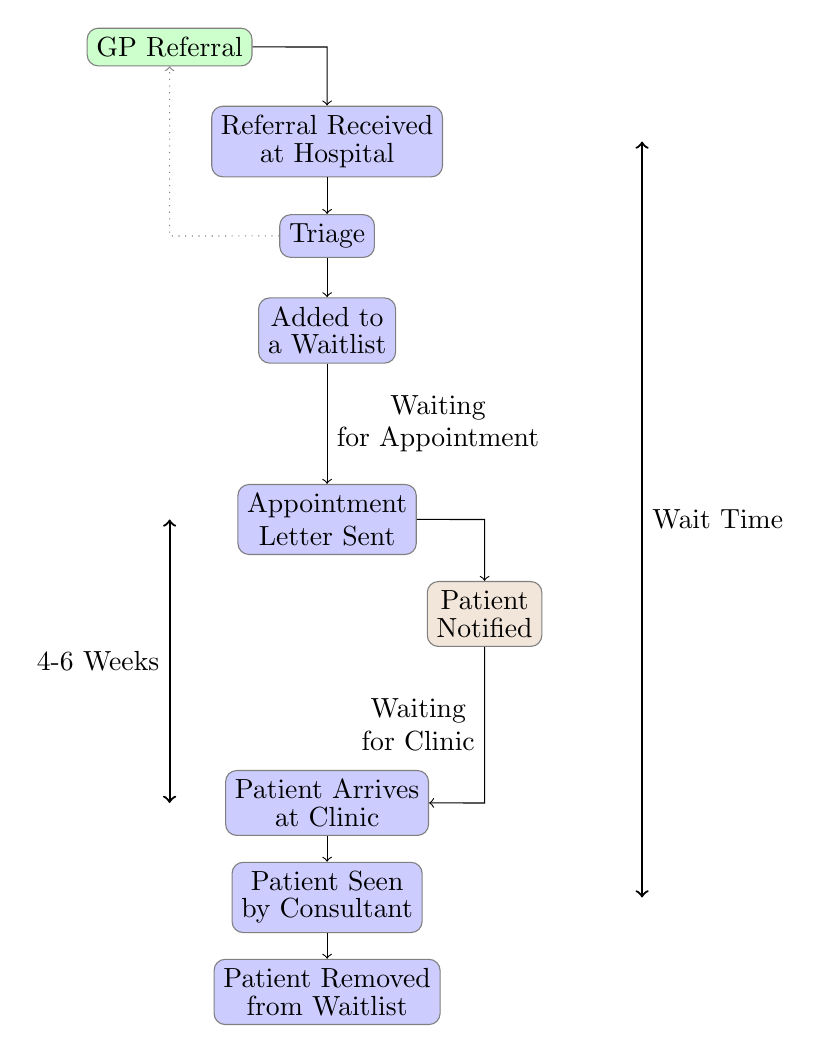
\begin{tikzpicture}[xscale=2,yscale=1.2]
  \node[draw=gray,fill=green!20,rounded corners] (referral) at (1,10) {GP Referral};
  \node[draw=gray,fill=blue!20,rounded corners] (receipt) at (2,9) {\shortstack{Referral Received\\at Hospital}};
  \node[draw=gray,fill=blue!20,rounded corners] (triage) at (2,8) {Triage};
  \node[draw=gray,fill=blue!20,rounded corners] (waitlist) at (2,7) {\shortstack{Added to\\a Waitlist}};
  \node[draw=gray,fill=blue!20,rounded corners] (appointment) at (2,5) {\shortstack{Appointment\\Letter Sent}};
  \node[draw=gray,fill=brown!20,rounded corners] (notified) at (3,4) {\shortstack{Patient\\Notified}};
  \node[draw=gray,fill=blue!20,rounded corners] (arrival) at (2,2) {\shortstack{Patient Arrives\\at Clinic}};
  \node[draw=gray,fill=blue!20,rounded corners] (seen) at (2,1) {\shortstack{Patient Seen\\by Consultant}};
  \node[draw=gray,fill=blue!20,rounded corners] (removed) at (2,0) {\shortstack{Patient Removed\\from Waitlist}};
  \draw[->] (referral) -- (2,10) -- (receipt);
  \draw[->] (receipt) -- (triage);
  \draw[->] (triage) -- (waitlist);
  \draw[->,dotted,gray] (triage) -- (1,8) -- (referral);
  \draw[->] (waitlist) -- node[right] {\shortstack{Waiting\\for Appointment}} (appointment);
  \draw[->] (appointment) -- (3,5) -- (notified);
  \draw[->] (notified) -- node[left] {\shortstack{Waiting\\for Clinic}} (3,2) -- (arrival);
  \draw[->] (arrival) -- (seen);
  \draw[->] (seen) -- (removed);
  \draw[<->,thick] (4,9) -- node[right] {Wait Time} (4,1);
  \draw[<->,thick] (1,5) -- node[left] {4-6 Weeks} (1,2);
\end{tikzpicture}
}

\end{frame}

\begin{frame}
\frametitle{National Waitlist Management Protocol (2017)}
\begin{tabular}{@{}c@{ }c@{ }c@{ }c@{ }c@{}}
\includegraphics[width=2cm]{images/addingtowaitlist} &
\includegraphics[width=2cm]{images/addingtoplannedprocedure} &
\includegraphics[width=2cm]{images/cancellationprocess} &
\includegraphics[width=2cm]{images/schedulingadmission} &
\includegraphics[width=2cm]{images/dnaprocess} \\
\includegraphics[width=2cm]{images/suspensionprocess} &
\includegraphics[width=2cm]{images/insourcingprocess} &
\includegraphics[width=2cm]{images/outsourcingprocess} &
\includegraphics[width=2cm]{images/validationprocess} &
\includegraphics[width=2cm]{images/removalprocess} 
\end{tabular}

\vspace{0.5cm}
{\scriptsize Inpatient/DayCase Process Shown, Outpatient Document Not Final}
\end{frame}

\begin{frame}
\frametitle{The Bad News}
\includegraphics[width=7cm]{images/newoutpatientswaitingdec2017}
{\scriptsize Data: NTPF}
\end{frame}


\begin{frame}
\frametitle{Patients Waiting: The Very Bad News}
%\includegraphics[width=9cm]{images/waitingband2}
\includegraphics[width=7cm]{images/newoutpatientswaitingbands}
{\scriptsize Data: NTPF}
\end{frame}

%% \begin{frame}
%% \frametitle{Patients Waiting: Age Groups}
%% \includegraphics[width=9cm]{images/waitingagegroup}
%% \end{frame}

\begin{frame}
\frametitle{KPI: Waiting Time Percentage}
\includegraphics[width=8cm]{images/kpiwaitingtimepercentagedec2017}
{\scriptsize Data: HSE}
\end{frame}

%% \begin{frame}
%% \frametitle{Outpatient Attendance}
%% \includegraphics[width=10cm]{images/attendance}
%% \end{frame}

%% \begin{frame}
%% \frametitle{Slow Uptake of Electronic Referrals}
%% \includegraphics[width=7cm]{images/referralnumbers}
%% \end{frame}

%% \begin{frame}
%% \frametitle{Patients Waiting: By Hospital}
%% \includegraphics[width=7cm]{images/standalone}
%% \end{frame}

\begin{frame}
\frametitle{A Near Universal Problem in Ireland}
\begin{tabular}{cc}
By Hospital &
\includegraphics[width=8cm]{images/byhospital}\\
By Speciality &
\includegraphics[width=8cm]{images/byspeciality}
\end{tabular}
\end{frame}

\begin{frame}
\frametitle{Heatmap: Where is the biggest problem?}
\includegraphics[width=11cm]{images/heatmap}
\end{frame}

\begin{frame}
\frametitle{Our Brief}
\begin{itemize}
\item Concentrate on Outpatients
\item Develop strategy for appointment decision making
\item What-if tool to understand the impact of decisions
\item Support current stakeholders
\item Not: Build automated appointment scheduling tool
\end{itemize}
\end{frame}

\begin{frame}
\frametitle{Project Roles}
\begin{itemize}
\item Data Analyst
\item Modeller
\item Outsourced Appointment Manager
\item Outsourced Process Owner
\item Hospital Waitlist Manager (part)
\item Hospital IT Manager (part)
\end{itemize}
\end{frame}


\begin{frame}
\frametitle{The Appointment Conundrum}
\begin{itemize}
\item We have to give ``routine'' appointment before knowing ``urgent'' demand
\item There is limited capacity
\item No overtime allowed (Croke Park agreement)
\item How much capacity to set aside for urgent cases?
\item How much overbooking is possible?
\end{itemize}
\end{frame}

\begin{frame}
\frametitle{Ways to Improve}
\begin{itemize}
\item Increase capacity
\item Reduce DNA (did not attend)
\item Decrease ratio return to new appointments
\item Move patients between consultants
\item Move patients between hospitals
\item Avoid unused slots
\item Fair treatment of all patients within same category
\end{itemize}
\end{frame}

\begin{frame}
\frametitle{Methodology}
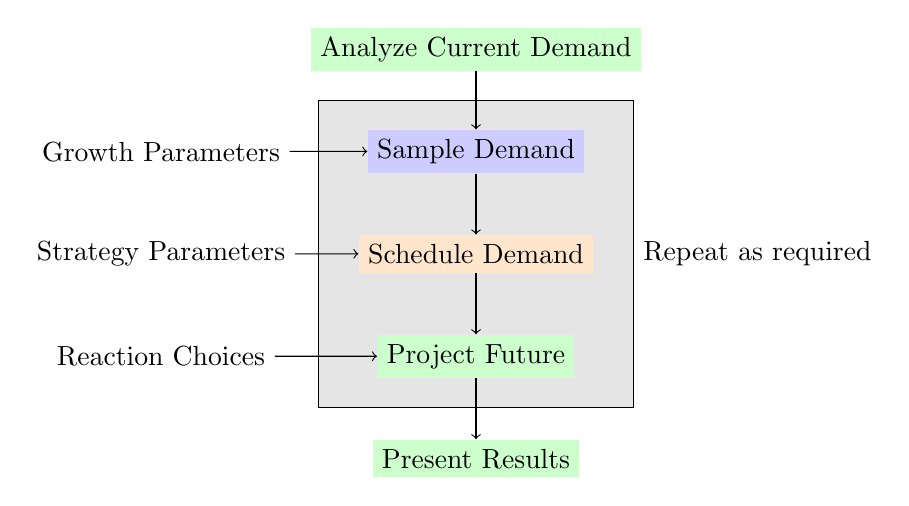
\begin{tikzpicture}[xscale=2,yscale=1.3]
  \draw[fill=black!10] (0,1.5) rectangle (2,4.5);
  \node[right] at (2,3) {Repeat as required};
  \node[fill=green!20] (analyse) at (1,5) {Analyze Current Demand};
  \node[fill=blue!20] (sample) at (1,4) {Sample Demand};
  \node (increase) at (-1,4) {Growth Parameters};
  \node (params) at (-1,3) {Strategy Parameters};
  \node (reaction) at (-1,2) {Reaction Choices};
  \node[fill=orange!20] (schedule) at (1,3) {Schedule Demand};
  \node[fill=green!20] (project) at (1,2) {Project Future};
  \node[fill=green!20] (present) at (1,1) {Present Results};
  \draw[->] (analyse) -- (sample);
  \draw[->] (increase) -- (sample);
  \draw[->] (sample) -- (schedule);
  \draw[->] (params) -- (schedule);
  \draw[->] (schedule) -- (project);
  \draw[->] (reaction) -- (project);
  \draw[->] (project) -- (present);
\end{tikzpicture}

\end{frame}

\begin{frame}
\frametitle{Demand Data (Not Public)}
\begin{tabular}{cc}
\shortstack{Received\\Per Day}&
\shortstack{Received\\Per Day of Week}\\
\includegraphics[width=4.5cm]{images/referralsperday} &
\includegraphics[width=4.5cm]{images/referralsdayofweek}
\end{tabular}

{\small
\begin{itemize}
\item Fitting distributions
\begin{itemize}
\item Poisson, not good fit
\item Negative Binomial
\end{itemize}
\item Limited Seasonality (unlike Emergency Department)
\end{itemize}
}
\end{frame}

\begin{frame}
\frametitle{Growth Parameters}
\begin{itemize}
\item Short/medium-term horizon (12-24 months)
\begin{itemize}
\item Keep demand constant
\item Increase with historical rates
\item Consider regional population increase 
\end{itemize}
\item More Complex:
\begin{itemize}
\item Age structure, birth rates
\item More appropriate for long-term demand forecast
\end{itemize}
\end{itemize}
\end{frame}

\begin{frame}
\frametitle{Waitlist/Clinic Model}
\scalebox{0.45}{
  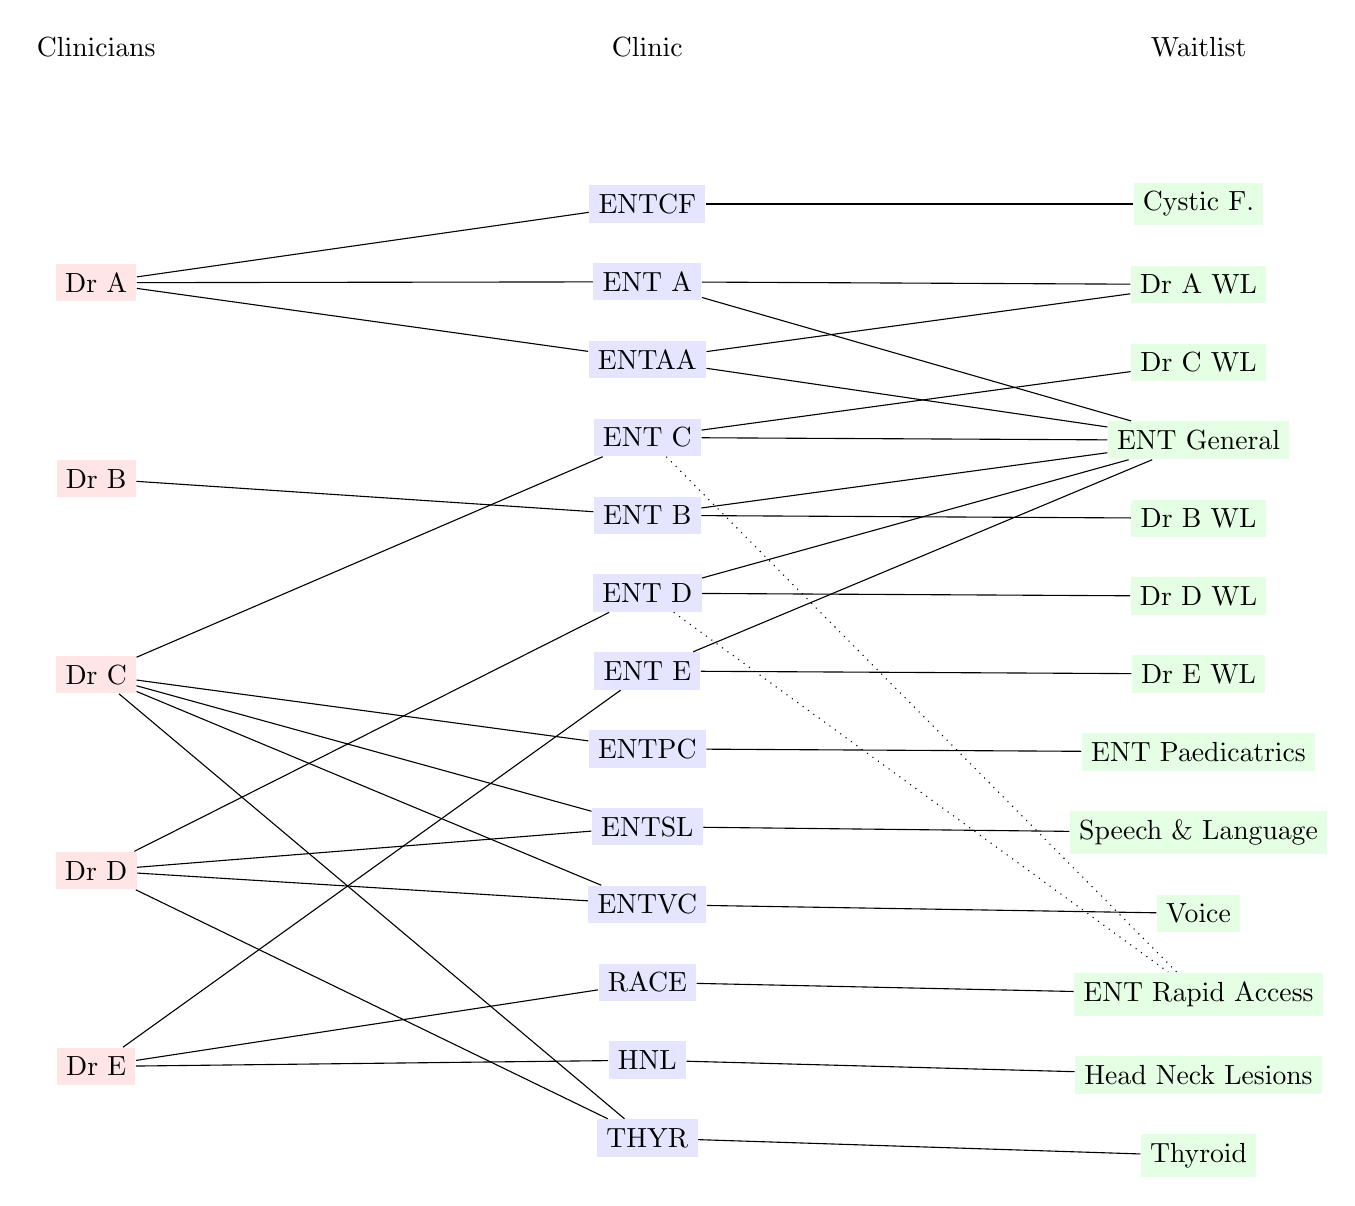
\begin{tikzpicture}
    \node at (0,12) {Clinicians};
    \node at (7,12) {Clinic};
    \node at (14,12) {Waitlist};
\node[fill=red!10] (smyth) at (0,9) {Dr A}; 
\node[fill=red!10, below = 2 cm of smyth] (mahesh)  {Dr B}; 
\node[fill=red!10, below = 2 cm of mahesh] (lang)  {Dr C}; 
\node[fill=red!10, below = 2 cm of lang] (skinner)  {Dr D}; 
\node[fill=red!10, below = 2 cm of skinner] (donnelly)  {Dr E}; 
\node[fill=blue!10] (entcf) at (7,10) {ENTCF}; 
\node[fill=blue!10, below = 0.5 cm of entcf ] (entds)  {ENT A}; 
\node[fill=blue!10, below = 0.5 cm of entds ] (entdx)  {ENTAA}; 
\node[fill=blue!10, below = 0.5 cm of entdx ] (entel)  {ENT C}; 
\node[fill=blue!10, below = 0.5 cm of entel ] (entmh)  {ENT B}; 
\node[fill=blue!10, below = 0.5 cm of entmh ] (entms)  {ENT D}; 
\node[fill=blue!10, below = 0.5 cm of entms ] (entmt)  {ENT E}; 
\node[fill=blue!10, below = 0.5 cm of entmt ] (entpc)  {ENTPC}; 
\node[fill=blue!10, below = 0.5 cm of entpc ] (entsl)  {ENTSL}; 
\node[fill=blue!10, below = 0.5 cm of entsl ] (entvc)  {ENTVC}; 
\node[fill=blue!10, below = 0.5 cm of entvc ] (race)  {RACE}; 
\node[fill=blue!10, below = 0.5 cm of race ] (skcl)  {HNL}; 
\node[fill=blue!10, below = 0.5 cm of skcl ] (thyr)  {THYR}; 
\node[fill=green!10] at (14,10) (cystic) {Cystic F.};
\node[fill=green!10, below= 0.5 cm of cystic]  (smyth_wl) {Dr A WL};
\node[fill=green!10, below= 0.5 cm of smyth_wl]  (lang_wl) {Dr C WL}; 
\node[fill=green!10, below= 0.5 cm of lang_wl]  (ent) {ENT General}; 
\node[fill=green!10, below= 0.5 cm of ent]  (mahesh_wl) {Dr B WL}; 
\node[fill=green!10, below= 0.5 cm of mahesh_wl]  (skinner_wl) {Dr D WL}; 
\node[fill=green!10, below= 0.5 cm of skinner_wl]  (donnelly_wl) {Dr E WL}; 
\node[fill=green!10, below= 0.5 cm of donnelly_wl]  (paed) {ENT Paedicatrics}; 
\node[fill=green!10, below= 0.5 cm of paed]  (speech) {Speech \& Language}; 
\node[fill=green!10, below= 0.5 cm of speech]  (voice) {Voice}; 
\node[fill=green!10, below= 0.5 cm of voice]  (rapid) {ENT Rapid Access}; 
\node[fill=green!10, below= 0.5 cm of rapid]  (lesion) {Head Neck Lesions}; 
\node[fill=green!10, below= 0.5 cm of lesion]  (thyroid) {Thyroid}; 
\draw[] (smyth) -- (entcf); 
\draw[] (smyth) -- (entds); 
\draw[] (smyth) -- (entdx); 
\draw[] (lang) -- (entel); 
\draw[] (lang) -- (entpc); 
\draw[] (lang) -- (entsl); 
\draw[] (lang) -- (entvc); 
\draw[] (lang) -- (thyr); 
\draw[] (mahesh) -- (entmh); 
\draw[] (skinner) -- (entms); 
\draw[] (skinner) -- (entsl); 
\draw[] (skinner) -- (thyr); 
\draw[] (donnelly) -- (entmt); 
\draw[] (donnelly) -- (race); 
\draw[] (donnelly) -- (skcl); 
\draw[] (entcf) -- (cystic); 
\draw[] (entds) -- (smyth_wl); 
\draw[] (entdx) -- (smyth_wl); 
\draw[] (entel) -- (lang_wl); 
\draw[] (entds) -- (ent); 
\draw[] (entdx) -- (ent); 
\draw[] (entel) -- (ent); 
\draw[] (entmh) -- (ent); 
\draw[] (entms) -- (ent); 
\draw[] (entmt) -- (ent); 
\draw[] (entmh) -- (mahesh_wl); 
\draw[] (entms) -- (skinner_wl); 
\draw[] (entmt) -- (donnelly_wl); 
\draw[] (entpc) -- (paed); 
\draw[] (entsl) -- (speech); 
\draw[] (entvc) -- (voice); 
\draw[] (race) -- (rapid); 
\draw[] (skcl) -- (lesion); 
\draw[] (thyr) -- (thyroid); 
\draw[dotted] (entel) -- (rapid); 
\draw[dotted] (entms) -- (rapid); 
\draw[] (skinner) -- (entvc);
\end{tikzpicture}
}

\end{frame}


\begin{frame}
\frametitle{Learning Capacity from Historical Data}
\includegraphics[width=10cm]{images/samplecliniccalendar}
{\small
\begin{itemize}
\item Repeat frequency
\item Capacity
\item Cancellation frequency
\item Replacement clinics
\end{itemize}
}
\end{frame}

\begin{frame}
\frametitle{Optimization Problem}
\begin{itemize}
\item Assign waiting patients to slots in clinics
\item Use appropriate clinic for given patient
\item Make appointments $k_p$ days in advance
\item Free and reuse slots when patients cancel
\item Reschedule patients when clinic cancelled
\item Do not change appointments otherwise
\item Reserve $u$ slots for urgent cases
\item Solved for each day
\end{itemize}
\end{frame}

\begin{frame}
\frametitle{Waitlist Actions}
\scalebox{0.55}{
  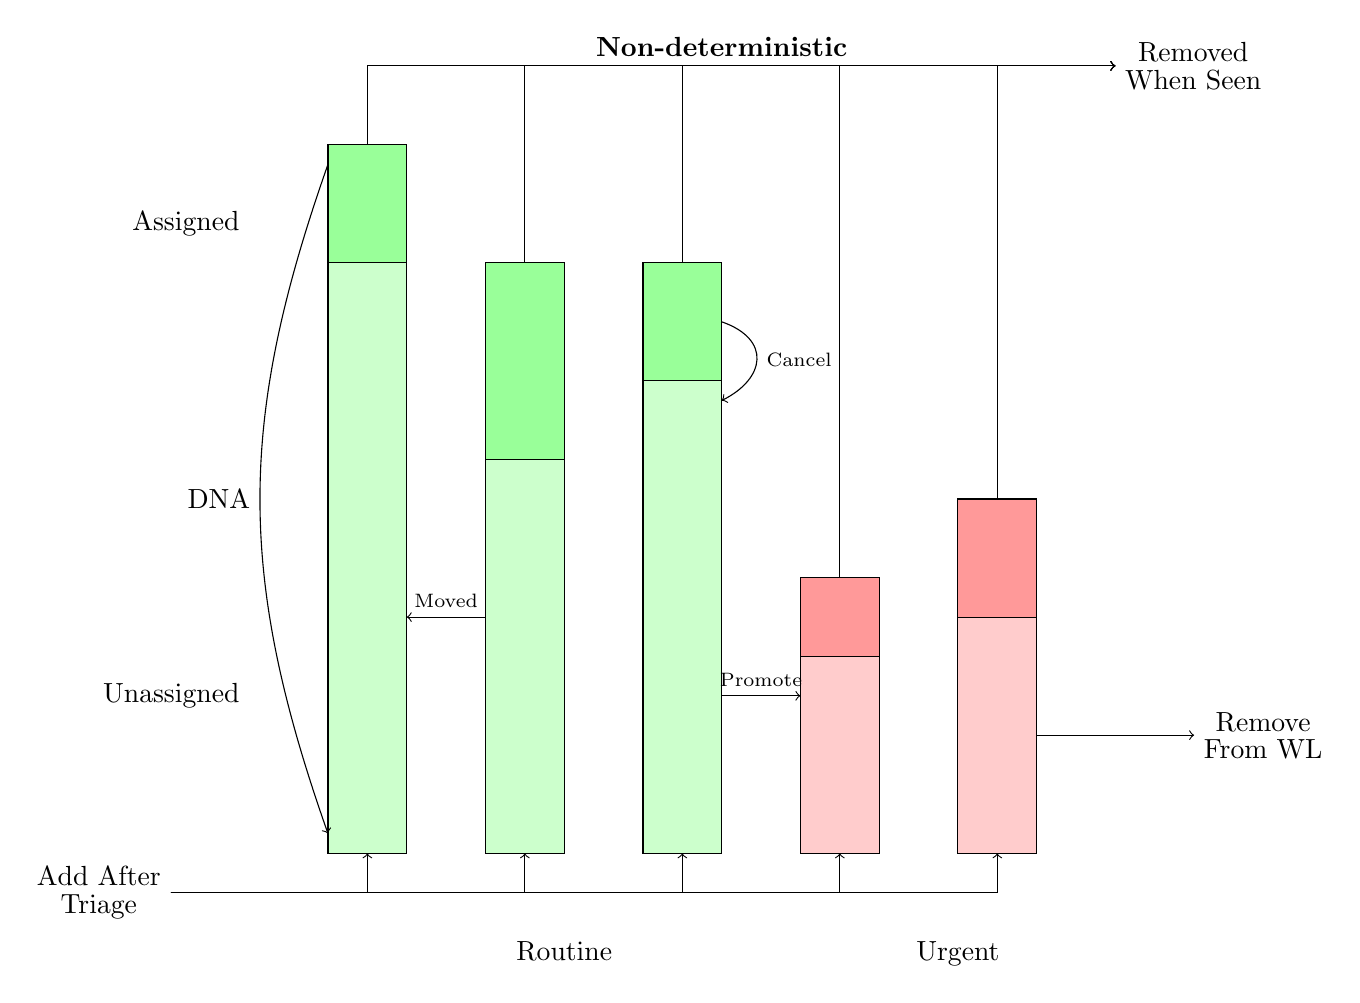
\begin{tikzpicture}[xscale=1,yscale=0.5]
  \draw[fill=green!20] (0,0) rectangle (1,15);
  \draw[fill=green!40] (0,15) rectangle (1,18);
  \draw[fill=green!20] (2,0) rectangle (3,10);
  \draw[fill=green!40] (2,10) rectangle (3,15);
  \draw[fill=green!20] (4,0) rectangle (5,12);
  \draw[fill=green!40] (4,12) rectangle (5,15);
  \draw[fill=red!20] (6,0) rectangle (7,5);
  \draw[fill=red!40] (6,5) rectangle (7,7);
  \draw[fill=red!20] (8,0) rectangle (9,6);
  \draw[fill=red!40] (8,6) rectangle (9,9);
  \node[below] at (3,-2) {Routine};
  \node[below] at (8,-2) {Urgent};
  \node[left] at (-1,4) {Unassigned};
  \node[left] at (-1,16) {Assigned};
  \draw[->] (-2,-1) -- (0.5,-1) -- (0.5,0);
  \draw[->] (-2,-1) -- (2.5,-1) -- (2.5,0);
  \draw[->] (-2,-1) -- (4.5,-1) -- (4.5,0);
  \draw[->] (-2,-1) -- (6.5,-1) -- (6.5,0);
  \draw[->] (-2,-1) -- (8.5,-1) -- (8.5,0);
  \node[left] at (-2,-1) {\shortstack{Add After\\Triage}};
  \draw[->] (0.5,18) -- (0.5,20) -- (10,20);
  \draw[->] (2.5,15) -- (2.5,20) -- (10,20);
  \draw[->] (4.5,15) -- (4.5,20) -- (10,20);
  \draw[->] (6.5,7) -- (6.5,20) -- (10,20);
  \draw[->] (8.5,9) -- (8.5,20) -- (10,20);
  \node[right] at (10,20) {\shortstack{Removed\\When Seen}};
  \node[above] at (5,20) {\textbf{Non-deterministic}};
  \draw[->] (0,17.5) to [out=260,in=100] node[left] {DNA} (0,0.5);
  \draw[->] (5,13.5) to [out=325,in=45] node[right] {\scriptsize Cancel} (5,11.5);
  \draw[->] (2,6) -- node[above] {\scriptsize Moved} (1,6);
  \draw[->] (5,4) -- node[above] {\scriptsize Promote} (6,4);
  \draw[->] (9,3) --  (11,3);
  \node[right] at (11,3) {\shortstack{Remove\\From WL}};
\end{tikzpicture}
}

\end{frame}

\begin{frame}
\frametitle{Clinic Allocation}
\scalebox{0.6}{
  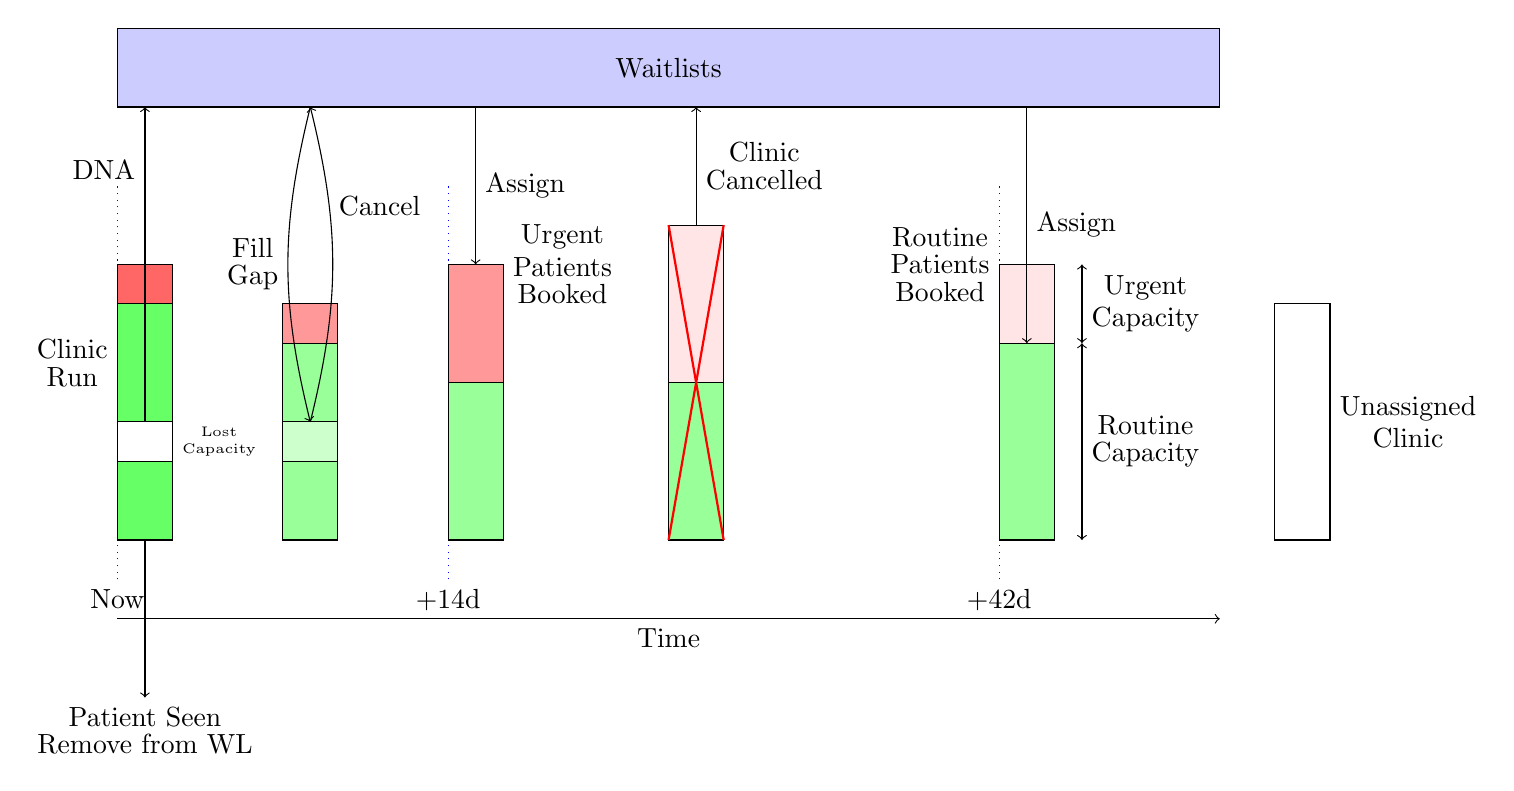
\begin{tikzpicture}[xscale=0.7,yscale=0.5]
    \draw[->](0,-2) --node[below] {Time} (20,-2);
    \draw[dotted,blue] (0,-1) -- (0,9);
    \draw[dotted,blue] (6,-1) -- (6,9);
    \draw[dotted,blue] (16,-1) -- (16,9);
    \node[below] at (0,-1) {Now};
    \node[below] at (6,-1) {+14d};
    \node[below] at (16,-1) {+42d};
    
    \draw[fill=green!60] (0,0) rectangle (1,6);
    \draw[fill=red!60] (0,6) rectangle (1,7);
    \node[left] at (0,4.5) {\shortstack{Clinic\\Run}};
    
    \draw[fill=green!40] (3,0) rectangle (4,5);
    \draw[fill=red!40] (3,5) rectangle (4,6);
    

    \draw[fill=green!40] (6,0) rectangle (7,4);
    \draw[fill=red!40] (6,4) rectangle (7,7);
    \node [right] at (7,7) {\shortstack{Urgent\\Patients\\Booked}};

    \draw[fill=green!40] (10,0) rectangle (11,4);
    \draw[fill=red!10] (10,4) rectangle (11,8);

    \draw[fill=green!40] (16,0) rectangle (17,5);
    \draw[fill=red!10] (16,5) rectangle (17,7);
    \node [left] at (16,7) {\shortstack{Routine\\Patients\\Booked}};

    \draw[fill=none,draw=black] (21,0) rectangle (22,6);
    \node[right] at (22,3) {\shortstack{Unassigned\\Clinic}};

    \draw[<->] (17.5,0) -- node[right] {\shortstack{Routine\\Capacity}} (17.5,5);
    \draw[<->] (17.5,5) -- node[right] {\shortstack{Urgent\\Capacity}} (17.5,7);

    \draw[fill=blue!20] (0,11) rectangle (20,13);
    \node at (10,12) {Waitlists};

    \draw[->] (16.5,11) -- node[right] {Assign} (16.5,5);
    \draw[->] (6.5,11) -- node[right] {Assign} (6.5,7);
    \draw[fill=white,draw=black] (0,2) rectangle(1,3);
    \node[right] at (1,2.5) {\tiny\shortstack{Lost\\Capacity}};
    \draw[->] (0.5,3) -- node[pos=0.8,left] {DNA} (0.5,11);
    \draw[->] (0.5,0) -- (0.5,-4);
    \node[below] at (0.5,-4) {\shortstack{Patient Seen\\Remove from WL}};

    \draw[fill=green!20] (3,2) rectangle (4,3);
    \draw[<-] (3.5,11) to [out=280,in=80] node[pos=0.3,right] {Cancel} (3.5,3);
    \draw[<-] (3.5,3) to [out=100,in=260] node[left] {\shortstack{Fill\\Gap}} (3.5,11);

    \draw[red,thick] (10,0) -- (11,8);
    \draw[red,thick] (11,0) -- (10,8);
    \draw[->,black] (10.5,8) -- node[right] {\shortstack{Clinic\\Cancelled}} (10.5,11);
  \end{tikzpicture}
}

\end{frame}

\begin{frame}
\frametitle{Baseline Analysis, Management View}
\includegraphics[width=11cm]{images/baseline}
\end{frame}

\begin{frame}
\frametitle{Scenario: Balance Patients Between Hospitals}
\includegraphics[width=11cm]{images/balanced}
\end{frame}

\begin{frame}
\frametitle{Scenario: Reduce DNA (Did not attend) to 5\%}
\includegraphics[width=11cm]{images/dna5percent}
\end{frame}

\begin{frame}
\frametitle{Scenario: Add Capacity}
\includegraphics[width=11cm]{images/drnew}
\end{frame}

\begin{frame}
\frametitle{Scenario: Add More Capacity}
\includegraphics[width=11cm]{images/drnew2}
\end{frame}

\begin{frame}
\frametitle{Status}
\begin{itemize}
\item Developed for industrial partner
\item Tested and evaluated at hospital
\item Actual data used, manual feed
\item Data integration issues unsolved
\item Difficult to find sponsor
\item Currently not continued
\end{itemize}
\end{frame}

\begin{frame}
\frametitle{The Need is Still There}
\includegraphics[width=8cm]{images/newoutpatientswaitingaug2018}
\end{frame}

%% \begin{frame}
%% \frametitle{Dashboard}
%% \includegraphics[width=10cm]{images/ntpf}
%% \end{frame}

%% \begin{frame}
%% \frametitle{Key Factor: Return/New Ratio}
%% \includegraphics[width=10cm]{images/kpireturnewratio}
%% \end{frame}

\begin{frame}
\frametitle{Summary}
\begin{itemize}
\item Presented case study from Irish health system
\item Strategy for outpatient appointments
\item Mix of analytics, simulation, and optimization
\item Nation-wide analysis of available data
\item What-if tool for selected departments
\end{itemize}
\end{frame}


\end{document}

\begin{frame}
\frametitle{}
\begin{itemize}
\item
\end{itemize}
\end{frame}

